%%=============================================================================
%% Methodologie
%%=============================================================================

\chapter{Methodologie}
\label{ch:methodologie}

%% TODO: Hoe ben je te werk gegaan? Verdeel je onderzoek in grote fasen, en
%% licht in elke fase toe welke stappen je gevolgd hebt. Verantwoord waarom je
%% op deze manier te werk gegaan bent. Je moet kunnen aantonen dat je de best
%% mogelijke manier toegepast hebt om een antwoord te vinden op de
%% onderzoeksvraag.

\section{Voorbereiding}
 Beide frontend applicaties maken gebruik van puur JavaScript, zonder het gebruik van externe libraries of frameworks zoals jQuery, React of Angular. Er werd enkel gebruik gemaakt van Webpack voor het bundelen van de code en het opzetten van een live development server om de applicatieontwikkeling te ondersteunen en van Babel voor het transpileren van JavaScript code. De applicatieontwikkeling bestaat uit vier delen: twee applicaties, één met een OOP aanpak en de ander met een FP aanpak, elk met een frontend en backend gedeelte. Er werd gekozen om beide aspecten te ontwikkelen zodat er ook op dat niveau een vergelijking mogelijk is tussen frontend en backend in zowel OOP als FP. Frontend technieken met backend vergelijken geeft geen goed beeld en enkel één van beide vergelijken geeft een te oppervlakkig beeld van de voordelen en nadelen van beide paradigma's. De applicatie die ontwikkeld werd is een applicatie voor drummers. Voor het uiteindelijke ontwikkelen van de applicatie werd eerst een UML \footnote{Unified Modeling Language: Modelleertaal die gebruikt wordt om het ontwerp van een applicatie te visualiseren} diagram aangemaakt om de verschillende klassen te illustreren \autocite{Booch2005}. Dit is voornamelijk voor de OOP applicatie. Een metronoom heeft een tempo en soort geluid en kan gestart en gestopt worden en kan 'tikken'. Een rudiment is een soort drumoefening en heeft een naam en een sticking (hoe de oefening moet uitgevoerd worden) en methodes voor het beheren van zijn practice sessions. Deze practice sessions geven aan hoe lang de drummer een bepaald rudiment heeft geoefend er voor hoe lang. 
 
\begin{figure}
    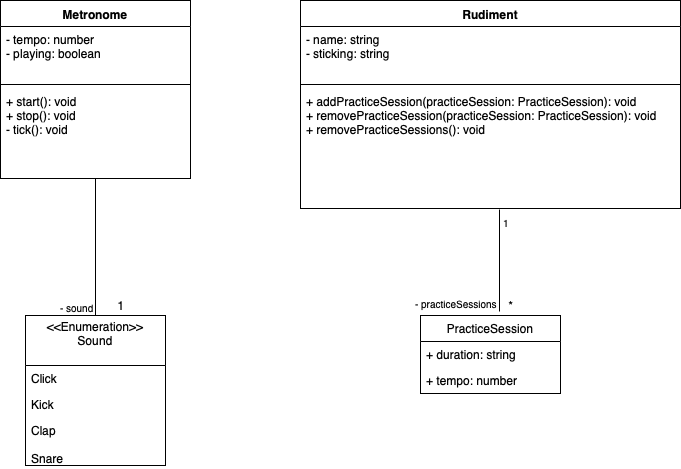
\includegraphics[width=\linewidth]{img/uml.png}
    \caption{UML Diagram voor de OOP applicatie}
    \label{fig:uml}
\end{figure}
 
 Voor de user interface van de applicatie komt er een metronoom aan te pas die ingesteld wordt aan de hand van een slider voor het tempo, een select veld voor het type geluid en een knop om de metronoom te starten en te stoppen. Verder is er ook een beheersysteem om de vooruitgang te volgen in bepaalde drumoefeningen, rudiments genaamd. Met een zoekveld kan er gezocht worden tussen de verschillende oefeningen. Wanneer er een oefening geselecteerd wordt en de metronoom wordt gestart dan zal de vooruitgang gevolgd worden en opgeslagen.

\begin{figure}
  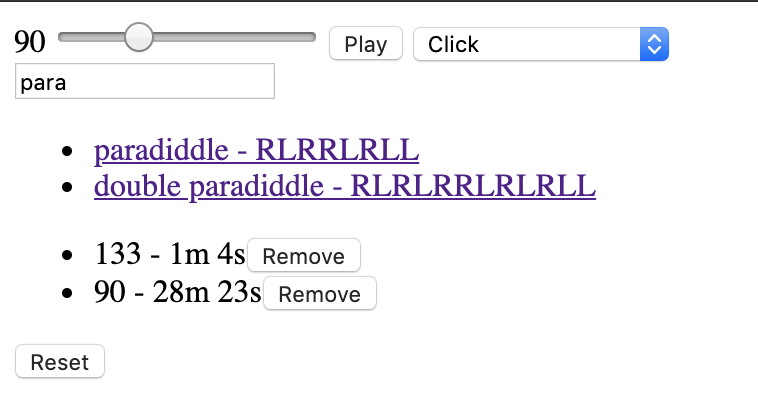
\includegraphics[width=\linewidth]{img/ui.png}
  \caption{User Interface van de applicatie}
  \label{fig:uml}
\end{figure}

 
 Analoog aan de frontend applicaties gebruikt de backend ook enkel puur JavaScript. Alle libraries die de ene applicatie gebruikt, gebruikt de andere applicatie ook, niet meer of minder. Dit maakt het mogelijk om een eerlijke en duidelijke vergelijking te maken. 

\section{Uitvoering}
Voor beide applicaties werd er eerst een standaard project aangemaakt met behulp van Webpack en Babel. Het opzetten van het project gebeurde met NPM, gebruik makende van het commando \textit{npm init}. Hierna werd aan beide projecten een configuratiebestand voor zowel Webpack als Babel toegevoegd waarin o.a. de configuratie staat voor de live development server. Vervolgens werd er een HTML pagina aangemaakt, deze is identiek voor beide applicaties. Enkel het JavaScript gedeelte verschilt. 

Voor de OOP frontend applicatie werden hiervoor eerst modellen gemaakt door middel van het creëren van klassen. Deze klassen zijn Metronome, Rudiment, PracticeSession en Stopwatch. Deze zullen de business logica van de applicatie bevatten. PracticeSession bevat enkel data (een tempo en een duration veld) maar de andere klassen bevatten ook methoden (zoals start en stop bij Metronome en hoe toevoegen of verwijderen van PracticeSessions bij Rudiment). Aangezien de data vanuit de backend komt in JSON formaat krijgen de klassen twee extra functies: fromJSON en toJSON. De fromJSON functie is een static functie om JSON naar een instantie van een klasse om te zetten. Daar deze static is kan de functie aangeroepen worden zonder eerst een instantie van deze klasse te maken (als JSON wordt opgehaald hebben we er immers nog geen). De tweede functie, toJSON, is een functie die de applicatie kan aanroepen op een object om deze om te zetten naar JSON. Deze functies zijn aanwezig bij zowel de Rudiment klasse als de PracticeSession klasse, dus de klassen waarvan er data naar en van de backend moet gestuurd worden. 

Voor de FP frontend applicatie werd alvast een sequence methode aangemaakt, deze vergemakkelijkt het samenstellen van (pure) functies die opeenvolgend worden uitgevoerd met het resultaat van de functie ervoor. Deze functie maakt ook gebruik van currying. Het eerste argument is een onbepaald aantal functies, het tweede argument is het argument waar de meegegeven functies op moeten worden toegepast. De reduce functie zorgt ervoor dat elke functie als argument het resultaat van de vorige functie meekrijgt, beginnende met de eerste functie die het tweede argument van de sequence functie met zich meekrijgt.

\begin{lstlisting}[language=HTML, caption=HTML pagina voor de frontend applicatie]
  <div>
    <div id="metronome">
      <label id="tempoLabel">60</label>
      <input type="range" id="tempoSlider" value="60" min="30" max="240" />
      <button id="metronomeButton">Play</button>
      <select id="soundSelect">
        <option>--select a sound--</option>
      </select>
    </div>
    <div id="rudiments">
      <input type="text" id="filter" placeholder="Filter rudiments..." />
      <ul id="rudimentList"></ul>
    </div>
    <div id="practiceSessions">
      <ul id="practiceSessionList"></ul>
    </div>
  </div>
  \end{lstlisting}

\begin{lstlisting}[caption=Sequence functie]
// een onbepaald aantal functies en argumenten worden meegegeven d.m.v. currying
const sequence = (...functions) => (...args) { 

  // de eerste functie en de rest van de functies worden opgeslagen in variabelen
  const [first, ...rest] = functions; 

  // reduce functie past elke functie toe op het resultaat van de vorige functie, beginnende met het resultaat van de eerste functie
  return rest.reduce((previousResult, currentFunction) => currentFunction(previousResult), first(args)); 
};
\end{lstlisting}

De beide backend applicaties maken gebruik van Node.js, Express, MongoDB en Mongoose om een REST API op te zetten. Analoog aan de frontend werd het project aangemaakt via het \textit{npm init} commando en werden de dependencies geïnstalleerd met behulp van NPM en het \textit{npm install --save *package*} commando. Het project bevat slechts één development dependency nl. Nodemon voor het opzetten van een live dev server die het development proces vergemakkelijkt door middel van live reloading wanneer de code wijzigt. 

\subsection{Frontend}
Deze subsectie handelt over de ontwikkeling van de frontend applicatie. Elk onderdeel van de frontend applicatie begint met een uitleg van de functionaliteit en vervolgens het ontwikkelproces van de OOP applicatie en gevolgd door het ontwikkelingsproces van de FP applicatie.

\subsubsection{Metronoom}
 Het eerste onderdeel dat werd geïmplementeerd was de metronoom. Voor de implementatie van de user interface moest een label continu geüpdatet worden aan de hand van de huidige waarde van een slider. Verder moest ook een knop geïmplementeerd worden om de metronoom te doen starten en stoppen en moest een select lijst opgevuld worden met de verschillende mogelijke geluiden van een metronoom. 
 
 Er werd eerst een MetronoomController gecreëerd, deze zal de koppeling vormen tussen View en Model. De Controller zal deze instantie van Metronome beheren zonder dat de View eraan kan (hier wordt er dus gebruik gemaakt van het facade pattern). Deze controller krijgt een aantal HTML elementen en maakt daar event listeners op aan zodat de Controller kan reageren op handelingen vanuit de user interface, i.e. het klikken op de start- en stopknop, het verplaatsen van de slider en het selecteren van een geluid. 

\begin{lstlisting}[caption=Afhandelen van een event - OOP]
// De controller luistert naar het input event van de slider   
tempoSlider.addEventListener('input', ({ target: { value: newTempo } }) => {
  // Het metronoom object wordt ingesteld met de nieuwe waarde
  this._metronome.tempo = newTempo;

  // Indien de metronoom aan het spelen is zal deze herstart worden zodat het nieuwe tempo wordt toegepast
  if (this._metronome.playing) {
    this._metronome.reset();
  }

  // Tenslotte wordt het nieuwe tempo weergegeven in de UI
  tempoLabel.innerText = newTempo;
});
 \end{lstlisting}

 De controller maakt hiervoor een instantie aan van de klasse Metronome, zodat het afhandelen gedelegeerd wordt aan dit object. 
 Aan de slider werd een event listener verbonden die het tempo van het Metronome object instelt en het label updatet zodat de user interface continu het juiste huidige tempo weergeeft. Duwen op de knop roept een methode op van de Metronome. Eerst kijkt de applicatie naar het \textit{playing} veld van het Metronome object, dit veld geeft aan of de metronoom al dan niet al aan het spelen is. Indien niet dan wordt de play methode aangeroepen en begint de metronoom te spelen door middel van de setInterval methode die tijdens elk interval een functie aanroept (in dit geval het tikken van de metronoom). Als de metronoom niet aan het spelen is dan wordt de stopfunctie aangeroepen, deze verwijdert het lopende interval. Bij het select input veld werd eerst de lijst aangevuld met de beschikbare opties. Een enumeratie (enum) houdt de verschillende mogelijk geluiden bij. Daar een enum type niet bestaat in puur JavaScript werd er gebruik gemaakt van de Object.freeze methode, deze sluit het meegegeven object af voor wijzigingen. Vervolgens itereert de controller over dit object door middel van een for...in loop, deze zal alle properties van het object doorlopen. Voor elke property maakt de controller dan een gepaste HTML node aan, in dit geval een option node. Daaraan hangt de controller dan tekst en hangt de volledige node dan aan het select input veld. Aan dit veld voegt de controller dan nog een event listener toe die bij het selecteren van een optie het sound veld van het Metronome object zal instellen met de gekozen waarde.
 
 \begin{lstlisting}[caption=Opvullen van het select veld - OOP]
   // iteratie d.m.v. een for..in loop
   for (const sound in Sound) {

      // aanmaken van het HTML option element met tekst
      const option = document.createElement('option');
      option.value = sound;
      const textnode = document.createTextNode(sound);
      option.appendChild(textnode);

      // toevoegen van dit element aan het select veld
      soundSelect.appendChild(option);
    }
 \end{lstlisting}

 Voor de FP applicatie bleek dit een moeilijk onderdeel om te implementeren. FP draait nu eenmaal rond pure functies, maar voor de metronoom is er geen input data en moet er ook niets geretourneerd worden. Dit onderdeel bestaat voornamelijk uit neveneffecten zoals het instellen van een veld van de user interface, het spelen en stoppen van de metronome etc. Dit is een zeer dynamische user interface, iets wat niet goed past bij een functionele aanpak. Analoog aan de OOP aanpak voegt de applicatie een event listener toe aan de slider zodat het label kan ingesteld worden met de juiste tempo waarde. Voor het spelen van de metronoom moet ook nog een regel van FP gebroken worden: immutability. Het spelen van de metronoom maakt weer gebruik van de setInterval functie. Dit interval moet bijgehouden worden zodat het bij het stoppen van de metronoom kan verwijderd worden. Hiervoor maakt de applicatie gebruik van een \textit{let} variabele, die muteerbaar is en dus een regel breekt van het functioneel programmeren. De staat van spelen van de metronoom houdt de applicatie ook niet bij, hiervoor is de applicatie afhankelijk van de tekst in de knop. Als deze op 'Play' staat dan is de metronoom niet aan het spelen, bij 'Stop' speelt deze dan weer wel. Dit maakt de applicatie echter afhankelijk van de View, wat geen best practice is aangezien deze beter losgekoppeld is van de logica. In tegenstelling tot het aanroepen van een Play functie op een metronoom object wordt er hier echter een algemene functie aangeroepen die een interval instelt door het tempo in BPM om te zetten naar milliseconden.
 
 \begin{lstlisting}[caption=Afhandelen van een event - FP]
// applicatie luistert naar het input event van de slider
tempoSlider.addEventListener('input', ({ target: { value: newTempo } }) => {

  // Het nieuwe tempo wordt weergegeven in de UI
  tempoLabel.innerText = newTempo;

  // als de interval variabele een waarde heeft dan wil dit zeggen dat de metronoom aan het spelen is
  if (interval) {
     clearInterval(interval);

     // het interval wordt opnieuw ingesteld, dit keer met het nieuwe gekozen tempo
     interval = setIntervalBPM(() => console.log(soundSelect.value), newTempo); 
  }
});

// hulpfunctie die het tempo in BPM zal omzetten naar milliseconden en daarmee setInterval aanroepen
function setIntervalBPM(callback, tempo) {
  return setInterval(callback, (60 / tempo) * 1000);
}
 \end{lstlisting}
 
 Het aanvullen van het select input veld met de verschillende geluidsopties is dan weer wel iets dat goed werkt binnen de FP applicatie. De applicatie itereert over de waarden van de makeshift enum en roept hierop de map functie aan. Aan de map functie wordt dan een pure functie meegegeven, createOption, die als input de string waarde van het geluid meekrijgt en als output een HTML element. Zo zal er voor elke waarde een HTML element aangemaakt worden en geeft de map functie dan een nieuwe lijst terug met deze elementen. Vervolgens vult de applicatie het select input veld op via de forEach functie die over de lijst itereert en een functie meekrijgt. Deze keer is dit geen pure functie, maar dit is een uitzondering die moet gemaakt worden om de View te kunnen wijzigen. Het aan elkaar rijgen van deze functies zorgt voor een declaratief statement dan de for..in loop in het OOP gedeelte. Hier zit de logica vooral in de functie die werd meegegeven aan map, terwijl bij het OOP gedeelte alle logica binnen de for..in loop zit.

 \begin{lstlisting}[caption=Opvullen van het select veld - FP]
// iteratie d.m.v. Object.values - deze overloopt de waarden van een object
// map gebruikt de meegegeven hulpfunctie om elke waarde om te zetten naar een HTML option element
// het resultaat van map wordt opnieuw overlopen m.b.v. forEach en deze zal de meegegeven functie gebruiken om het select veld aan te vullen
Object.values(Sound)
  .map(createOption)
  .forEach(el => soundSelect.appendChild(el));
// deze functies werden aan elkaar geregen zodat de tussenresultaten niet telkens in een variabele moeten opgeslagen worden

// hulpfunctie die een HTML option element teruggeeft
function createOption(value) {
  const optionEl = document.createElement('option');
  optionEl.value = value;
  const textNode = document.createTextNode(value);
  optionEl.appendChild(textNode);
  return optionEl;
}
 \end{lstlisting}

 \subsubsection{Lijst van Rudiments}
 Dit onderdeel bestaat uit een lijst van rudiments met een tekstveld waarop de lijst kan gefilterd worden. Hiervoor staat in de HTML een input tekstveld klaar en een leeg HTML lijstelement (ul). 
 
 Om in de OOP applicatie deze lijst van rudiments te beheren werd er opnieuw een controller gemaakt, RudimentController, die de rudiments zal opvragen van de backend en bijhouden. De controller krijgt het HTML lijstelement mee via de constructor en kan zo hier de aparte elementen voor elk rudiment aanhangen. Dit gebeurt via een showRudiments functie die over de lijst van rudiments zal itereren en per rudiment een HTML element aanmaken. Vervolgens hangt de controller deze elementen aan het lege HTML lijstelement dat hij meekreeg via zijn constructor. Voor de implementatie van de filter werd er een eventlistener toegevoegd aan het input tekstveld. Bij het veranderen van de input (dus wanneer er getypt wordt bv.) zal de applicatie de showRudiments functie opnieuw aanroepen. Deze wordt werd uitgebreid met een filter argument en nog een extra instructie die voor het aanmaken van de elementen eerst nog over de lijst itereert en de naam van het rudiment vergelijk met de tekst van de filter. Als de filtertekst voorkomt in de naam dan zal het rudiment toegevoegd worden aan een filteredRudiments array. De controller itereert dan over deze array zodat de View steeds de juiste rudiments toont op basis van de filtertekst in het input veld. 
 
\begin{lstlisting}[caption=Filteren van de rudiments - OOP]
// initialiseren van een array waarin de gefilterde rudiments worden opgeslagen
let filteredRudiments = [];

// iteratie d.m.v. for..in
for (let rudiment in this._rudiments) {
  // if statement bepaalt a.d.h.v. de filter of rudiment bij de gefilterde rudiments hoort
  if (rudiment.name.indexOf(filter) >= 0) {
    filteredRudiments.push(rudiment);
  }
}

for (let filteredRudiment in filteredRudiments) {
  // aanmaken van een HTML lijst element met tekst
  const listEl = document.createElement('li');
  const textNode = document.createTextNode(
    `${rudiment.name} - ${rudiment.sticking}`
  );
  listEl.appendChild(textNode);

  // lijst element toevoegen 
  this._rudimentListNode.appendChild(listEl);
}
\end{lstlisting}

 Het ophalen van de rudiments gebeurt via de fetch functie. Die functie verwacht een url en eventuele opties om de request te configureren. Om alle rudiments op te halen is hier enkel een url nodig. De RudimentController haalt deze rudiments op via een get request en zet de verkregen rudiments om van JSON naar objecten van de Rudiment klasse. Deze objecten zal de RudimentController bijhouden zodat er bij het filteren niet telkens opnieuw een netwerk call moet gebeuren.

De implementatie van dit onderdeel verreist het verwerken van een lijst met data, wat een sterkte is van functioneel programmeren. Voor het opvullen van het HTML lijstelement gebruiken we de sequence methode, deze zal een reeks functies uitvoeren met als beginnend argument een lijst data die rudiments bevat. Als eerste functie roept geeft de applicatie een getItemNodes functie mee. Deze methode maakt gebruik van currying zodat er eerst een aantal argumenten kunnen meegeven worden. De functie zal telkens opnieuw een functie teruggeven tot de applicatie de lijst van rudiments meegeeft, waarna de functie het echte werk doet met behulp van de voorgaande argumenten. Als eerste argument krijgt getItemNodes een mapFunctie mee die zal bepalen hoe elk item gemapt zal worden naar een HTML element. Voor deze mapFunctie geeft de applicatie de functie createRudimentListNode mee, deze verwacht als argument een rudiment en maakt hiervoor de nodige HTML elementen aan en geeft deze dan terug. Voorlopig is dit een lijstelement dat een tekstnode bevat waarin de details van het rudiment staan (naam en sticking). Als tweede argument voor de sequence functie geeft de applicatie de appendToDomElement functie mee. Deze maakt weer gebruik van currying en verwacht als eerste argument een DOM element waaraan het items zal aan toevoegen. Deze items zijn dan ook het tweede argument van deze functie. De sequence functie met de argument getItemNodes en appendToDomElement geeft dan opnieuw een functie terug die het beginnende argument verwacht, dit is de lijst met rudiments. Vervolgens zal deze lijst doorgegeven worden aan de getItemNodes functie die zijn mapFunctie argument zal toepassen op deze items en het resultaat retourneren. Dit resultaat, de lijst van HTML elementen, wordt op zijn beurt doorgegeven aan de appendToDomElement zodat de functie deze elementen toevoegt aan zijn DOM element argument. Deze compositie van functies is makkelijk herbruikbaar en zal dan ook hergebruikt worden voor het volgende onderdeel. Vervolgens werd er een event listener toegevoegd aan het input tekstveld. Deze zal opnieuw gebruik maken van de sequence functie met als argumenten getItemNodes en appendToDomElement maar deze argumenten worden voorafgegaan door de filterList functie die de rudiments zal filteren.

\begin{lstlisting}[caption=Filteren van de rudiments - FP]
// het filter tekstveld wordt opgehaald uit het DOM
// aan dit tekstveld wordt vervolgens een event listener toegevoegd
// het afhandelen van dit event gebeurt via de sequence functie
document
  .getElementById('filter')
  .addEventListener('input', ({ target: { value: filterText } }) => {
    sequence(
      filterList(filterText), // lijst filteren o.b.v. meegegeven tekst
      getItemNodes( // het aanmaken van de HTML elementen
        createRudimentListNode(
          onRudimentClick(practiceSessions, NO_SESSIONS)
        )
      ),
      appendToDOMElement(rudimentList) // HTML elementen toevoegen aan DOM
    )(...rudiments);
});
  \end{lstlisting}


Om de data op te halen vanuit de backend maakt de applicatie gebruik van de get hulpfunctie. Deze functie roept de fetch functie aan en vervolgens de json functie van diens respons zodat deze code niets steeds herhaald moet worden. Om ervoor te zorgen dat er niet steeds nieuwe netwerk calls nodig zijn stopt de applicatie de rudiments wel in een variabele, hoewel dit tegenstrijdig is met het immutability principe aangezien deze variabele eerst vooraf gedefinieerd moet worden en later gemuteerd door de rudiments eraan toe te kennen.

 \subsubsection{Lijst van Practice Sessions}
 Deze functionaliteit omvat opnieuw het weergeven van een lijst maar deze keer geen lijst waarop gefilterd kan worden maar een lijst die het mogelijk maakt om items aan toe te voegen en te verwijderen. Deze items omvatten sessies die het tempo tonen en tijdsduur ervan tonen. Deze sessies horen bij een rudiment en de gebruiker kan ze één voor één verwijderen of alle sessies verwijderen voor één rudiment. De practice sessions moeten getoond worden wanneer een rudiment geselecteerd wordt zodat zijn bijhorende practice sessions in de lijst worden weergegeven.

Analoog aan het vorige onderdeel werd voor de OOP applicatie opnieuw een controller gemaakt, de PracticeSessionController. De constructor van deze controller verwacht deze keer geen leeg HTML lijst element maar een gewoon HTML div element. De controller maakt in zijn constructor dan zelf een lijstelement aan dat hij zal toevoegen aan het div element. Net zoals voorgaand onderdeel bevat de controller een showPracticeSession functie, ditmaal met als argument een lijst van practice sessions. Deze lijst zal opnieuw doorlopen worden en per practice session maakt de controller een HTML element aan dat zal worden toegevoegd aan het HTML lijst element. Als de lijst leeg is dan voegt de controller een gepaste tekst toe aan het div element, vandaar dat deze implementatie iets anders is dan het vorige onderdeel. Voor het selecteren van een rudiment werd een eventlistener toegevoegd aan de RudimentController. Door middel van het gebruik van overerving breidt de controller dan de klasse EventTarget uit zodat deze zelf events kan sturen die door zijn listeners kunnen ontvangen worden. Vervolgens werd de showRudiments functie aangepast door aan een lijstelement nog een anchorelement toe te voegen. Dit zorgt ervoor dat er op een rudiment lijstelement kan geklikt worden. Bij een klik zal de RudimentController dan een event uitsturen die het desbetreffende rudiment meegeeft. De applicatie zal dan op dit event reageren door de practice sessions te tonen van het meegegeven rudiment. Bij elke klik op een rudiment geeft de applicatie dan de juiste lijst van practice sessions weer, of een gepaste tekst indien het rudiment geen practice sessions zou hebben. Het ophalen van de practice sessions gebeurt via een get request die de id van het geselecteerde rudiment zal meegeven zodat de backend de juiste practice sessions kan teruggeven.  

Om dit onderdeel te implementeren in de FP applicatie werden de functies getItemNodes en appendToDomElement van vorig onderdeel hergebruikt. Het argument dat de applicatie meegeeft aan getItemNodes is ditmaal een functie die een practice session zal omzetten naar een gepast HTML element. Dit omzetten en toevoegen van elementen roept de applicatie in de functie onRudimentClick. Deze gecurryde methode verwacht als eerste argument een HTML element om de lijst van practice session elementen aan toe te voegen en een placeholder om weer te geven indien er het geselecteerde rudiment geen practice sessions zou bevatten. De functie zal bij elke aanroep het meegegeven HTML element leegmaken zodat de applicatie telkens de juiste data kan tonen zonder dat de vorige data nog aanwezig is. Als laatste argument om de functie mee aan te roepen volgt de practice sessions data lijst. Als deze lijst niet leeg is zal de de functie zelf een HTML lijst element creëren en zal de functie vervolgens over de data lijst itereren en de gepaste HTML elementen aanmaken om deze vervolgens toe te voegen aan het gecreëerde HTML lijst element. Dit element wordt dan op diens beurt toegevoegd aan het HTML element dat als eerste argument werd meegegeven aan de functie. Indien de data lijst leeg blijkt te zijn of niet werd meegegeven maakt de functie een HTML paragraaf element aan die als de tekst het meegegeven placeholder argument zal bevatten. In dit geval is dit een boodschap die vermeldt dat er voor het geselecteerde rudiment nog geen practice sessions zijn. Om de onRudimentClick functie te gebruiken in de applicatie werd de createRudimentListNode functie aangepast. Hiervoor werd er opnieuw currying toegepast zodat deze functie als eerste argument nu een onClick methode verwacht. Verder maakt de createRudimentListNode nu een anchor HTML element aan zodat als er op geklikt wordt de anchor de meegegeven onClick methode aanroept, in dit geval is dit de onRudimentClick methode. Analoog aan de OOP applicatie wordt het anchor element rond de beschrijving van het rudiment gezet zodat erop geklikt kan worden zodat de applicatie de bijhorende practice sessions van het rudiment weergeeft of een gepaste tekst indien het geselecteerde rudiment geen practice sessions bevat. Het ophalen van de practice sessions gebeurt in de onRudimentClick functie. Deze zal het id van het meegegeven rudiment gebruiken om via een get request de juiste practice sessions op te halen uit de backend.

\subsection{Backend}
\subsubsection{OOP}
Alhoewel de OOP backend applicatie geen klassen definieert werkt deze toch volgens het OOP principe. De applicatie past ook het MVC pattern toe door middel van het gebruik van controllers aan wie het ophalen en beheren van data wordt gedelegeerd. Voor het gebruik van de MongoDB databank werden schema's gemaakt die de eigenschappen van een document bepalen, gelijkaardig aan het definieren van een klasse (maar zonder methoden uiteraard, enkel met data). Voor het aanspreken van deze methoden van de controllers definieert de applicatie enkel routes, de /rudiment routes delegeert deze dan aan de rudimentController terwijl het aanspreken van de /practiceSessions routes zullen gedelegeerd worden aan de practiceSessionController. De rudimentController beheert ook deels de practice sessions maar dan die van een specifiek rudiment dat wordt opgevraagd. Het opvragen van zo'n specifiek rudiment gebeurt via de /rudiment/:rudimentId route en diens practice sessions kunnen dan opgevraagd worden door /practiceSessions aan die route toe te voegen. Ophalen van de rudiments en practice sessions gebeurt via get requests, het toevoegen van practice sessions via post requests en het verwijderen van deze gebeurt door delete requests. De data die de applicatie meegeeft en meekrijgt via deze requests staat in JSON formaat. De structuur voor het voldoen aan een request is redelijk vast, de backend spreekt voor de aangesproken route een gepaste methode aan op een controller klasse en deze methode roept op diens beurt één of meerdere functies aan op één of meerdere collecties uit de MongoDB databank. Verder maakt de applicatie ook nog gebruik van overerving. Beide controller klassen breiden een algemene Controller klasse uit. Van deze klasse zelf kan geen instantie gemaakt worden, net zoals een abstracte klasse, alleen is dit in principe geen echte abstracte klasse aangezien dit concept niet bestaat in puur JavaScript. Deze algemene klasse bevat al 3 methodes: getAll, getById en add. Dit zijn veel voorkomende methodes waarvan de implementatie steeds dezelfde is. Deze methoden hangen alleen af van een Mongoose Model zodat de juiste collectie uit de MongoDB databank kan gebruikt worden. Het model geeft de gespecialiseerde controller klasse mee in zijn constructor door dit mee te geven aan de super functie. Deze super functie roept de constructor van de superklasse aan en stelt zo het model in bij de superklasse. Zo geeft de RudimentController het Rudiment model mee in zijn constructor. Wanneer de applicatie de getAll functie aanroept op de RudimentController dan zal deze functie gebruik maken van het Rudiment model. Verder hebben beide controllers ook nog functies die eigen zijn aan die klasse en dus niet hergebruikt kunnen worden.

\begin{lstlisting}[caption=Afhandelen van de rudiments route - OOP]
// === Route === //
 app
    .route('/rudiments') // bepalen van de route
    .get(async (req, res) => { // afhandelen
      try {
        // delegeren naar RudimentController object
        const rudiments = await rudimentController.getAll();
        res.json(rudiments);
      } catch (err) {
        res.send(err);
      }
    })

// === Aangeroepen klassen === //
// abstracte klasse 
class Controller {
  constructor(model) {
    if (!model) {
      throw new Error('Cannot instantiate this object directly');
    }
    this._model = model;
  }

  // methode die een find operatie uitvoert op het Mongoose model waarmee het object werd aangemaakt
  async getAll() {
    return new Promise((resolve, reject) => {
      this._model.find({}, (err, data) => {
        if (err) reject(err);
        resolve(data);
      });
    });
  }
}

// Bij het aanmaken van een RudimentController zal deze de constructor van Controller aanroepen en het Rudiment model meegeven
class RudimentController extends Controller {
  constructor() {
    super(Rudiment);
  }
}
\end{lstlisting}

\subsubsection{FP}
Waar de routes bij de OOP applicatie de afhandeling voor een request overdragen aan een Controller, gebeurt dit bij de FP backend via het samenstellen van functies. Zo definieert de applicatie een aantal basis functies die dan hergebruikt kunnen worden in specifiekere functies. Deze gecurry'de basisfuncties zijn voor het ophalen, wijzigen, toevoegen en verwijderen van documenten in de MongoDB databank en verwachten telkens als eerste argument het Mongoose Model zodat deze functies kunnen toegepast worden op de juiste collectie in de databank. Deze functies zijn dan nog eens opgedeeld in het beheren van alle documenten in een collectie, één document dat via het id wordt opgehaald of één of meerdere documenten die worden opgehaald via een documentquery. Met deze basisfuncties definieert de backend dan specifieke functies om effectief rudiments of practice sessions te beheren. Het beheren van deze documenten in de databanken is uiteraard een neveneffect en dus geen gewenste handeling binnen het functioneel programmeren. Daarom stopt de applicatie deze handelingen in een Promise object. Dit zorgt ervoor dat het neveneffect zich niet meteen voordoet maar slechts wanneer via await de desbetreffende functie wordt aangeroepen. Op deze manier is er wel nog een soort van controle over het het uitvoeren van dit neveneffect. Verder definieert de applicatie ook nog enkel hulpfuncties om wat boilerplate code te verminderen, zoals voor het afhandelen van een binnenkomende request (er wordt ofwel JSON ofwel een foutmelding teruggestuurd) en voor het afhandelen van een respons vanuit de databank (een Promise moet geweigerd worden bij een foutmelding en opgelost worden bij het terugkrijgen van een resultaat).

\begin{lstlisting}[caption=Afhandelen van de rudiments route - FP]
// === Route === //
app
  .route('/rudiments') // bepalen van de route
  .get(handleRequestAndResponse(getAllRudiments)); // afhandeling


// === Hulpfuncties === //
// deze hulpfunctie stuurt het resultaat van een endpoint request terug als JSON of stuurt een error terug indien deze zich voordoet
const handleRequestAndResponse = endpoint => async (req, res) => {
  try {
    const result = await endpoint();
    res.json(result);
  } catch (err) {
    res.send(err);
  }
};


const getAllRudiments = () => getAll(Rudiment);

// deze functie verwacht een Mongoose model om een find operatie op uit te voeren
const getAll = model =>
  new Promise((resolve, reject) => {
    model.find({}, handleDbResponse(resolve, reject));
  });


\end{lstlisting}

\section{Resultaten}
\subsection{Lijnen code}
Om het aantal lijnen code te meten werd enkel gekeken naar de JavaScript bestanden zonder geïmporteerde libraries (node\_modules). De HTML is immers hetzelfde bij beide applicaties en er is geen styling toegevoegd geweest. Beide applicaties maakten gebruik van de Prettier extensie in VSCode om code te formatteren, dit zorgt voor consistentie in de lijnen code. De lijnen werden geteld via een bash commando. 

\begin{lstlisting}[caption=Bash commando]
    find . -name '*.js' | xargs wc -l
 \end{lstlisting}

 De frontend in functioneel programmeren stijl bestaat uit 288 lijnen verdeeld over 7 bestanden. Opmerkelijk hieraan is dat de meeste lijnen zich in de index.js bevinden, dus het eerste script dat de applicatie uitvoert. Deze stelt de werking van de applicatie in elkaar door andere gedefinieerde functies te gebruiken en op die manier de functionaliteit van de volledige applicatie uit te bouwen. Dit samenstellen van functies zorgt er echter voor dat de code minder leesbaar wordt.

 \begin{lstlisting}[caption=FP frontend aantal code]
    140 ./index.js
    24 ./utils.js
    49 ./modules/rudiment.js
    40 ./modules/practiceSession.js
    15 ./modules/components.js
     3 ./modules/metronome.js
    17 ./modules/network.js
   288 total
 \end{lstlisting}

De frontend in object-geörienteerde stijl bestaat daarentegen uit 475 lijnen verdeeld over 9 bestanden. In tegenstelling tot de FP frontend bevat het index.js bestand nu slechts 74 lijnen, bijna de helft van de lijnen van het index.js bestand uit de FP frontend. Een verklaring hiervoor is dat de logica vooral weggestopt zit in de klassen. Het enige dat het index.js script moet doen is de juiste klasse aanspreken voor een bepaalde functionaliteit, de klasse zal dit dan verder afhandelen. Dit zorgt ervoor dat het hoofdscript van de applicatie makkelijk leesbaar is, zeker als de klassen objecten voorstellen uit het echte leven want dat zorgt voor een duidelijk beeld van de verschillende functionaliteiten.

 \begin{lstlisting}[caption=OOP frontend aantal code]
    49 ./util/networkRequest.js
    74 ./index.js
    42 ./models/rudiment.js
    30 ./models/practiceSession.js
    67 ./models/metronome.js
    22 ./models/stopwatch.js
    54 ./controllers/metronomeController.js
    85 ./controllers/rudimentController.js
    52 ./controllers/practiceSessionController.js
    475 total
 \end{lstlisting}

 De backend voor functioneel programmeren bestaat uit 276 lijnen code verdeeld over 12 bestanden. Het route.js script is waar de omzetting gebeurt van http request route naar het aanroepen van de juiste functies om aan die request te voldoen. Dit script zal ,net als bij het index.js script uit de frontend, verschillende functies combineren om aan de gewenste functionaliteit te komen.

 \begin{lstlisting}[caption=FP backend aantal code]
    23 ./index.js
    57 ./routes.js
    11 ./api/endpoints/post.js
    14 ./api/endpoints/put.js
    16 ./api/endpoints/delete.js
    22 ./api/endpoints/get.js
     8 ./api/util/handleDbResponse.js
    12 ./api/util/handleRequestAndResponse.js
    19 ./api/models/rudimentModel.js
    17 ./api/models/practiceSessionModel.js
    10 ./api/modules/practiceSessions.js
    67 ./api/modules/rudiments.js
   276 total 
\end{lstlisting}

De backend voor functioneel programmeren bestaat uit 273 lijnen code verdeeld over 12 bestanden. Het route.js script heeft in dit geval meer lijnen code dan dat bij de FP backend. Dit komt doordat er per route code voor het afhandelen van de requests, responses en afhandelen van de asynchrone functies wordt herhaald terwijl de applicatie van de FP backend dit afhandelt via hulpfuncties. Dit is uiteraard ook mogelijk om te doen in een OOP applicatie, maar dit is vooral iets typisch bij een FP applicatie door samenstelling van functies.

 \begin{lstlisting}[caption=OOP backend aantal code]
    23 ./index.js
    94 ./routes.js
    19 ./api/models/rudimentModel.js
    17 ./api/models/practiceSessionModel.js
    36 ./api/controllers/controller.js
    63 ./api/controllers/rudimentController.js
    21 ./api/controllers/practiceSessionController.js
    273 total
 \end{lstlisting}

 \subsection{Performantie}
In dit onderdeel werd er gekeken naar de tijd die nodig is voor het inladen van de JavaScript code in een browser en de nodige tijd voor het terugkrijgen van een resultaat uit de backend. Voor het inladen van de JavaScript code werd er gekeken naar hoe snel de main.bundle.js wordt ingeladen. Dit is een bundeling van de volledige code die gebeurt door webpack. Om de laadtijd te kennen werd gebruik gemaakt van de Chrome Developer Tools. Voor de laadtijd van de backend requests werd Postman gebruikt. Elke meting werd 30 keer uitgevoerd om de spreiding ervan te kunnen meten.

\begin{figure}
    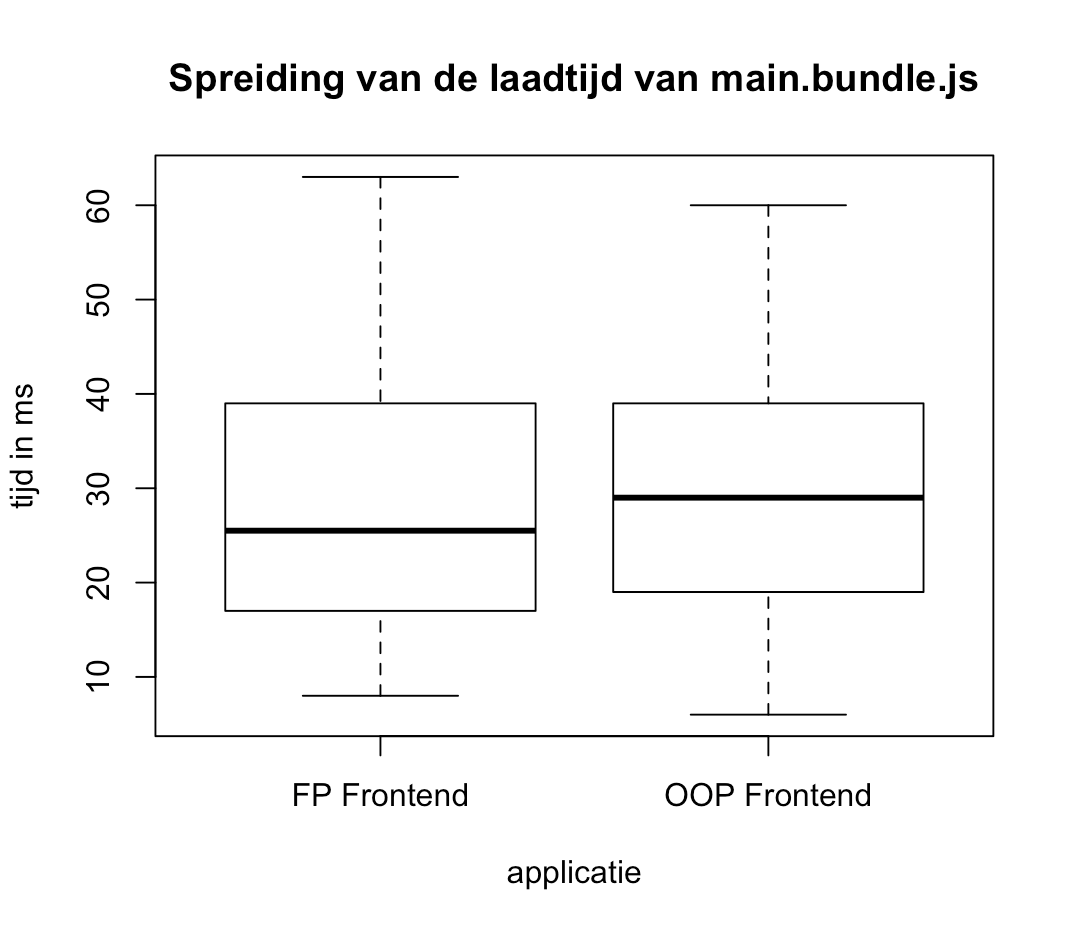
\includegraphics[width=\linewidth]{img/performantie-frontend.png}
    \caption{Performantie Frontend}
    \label{fig:performantiebackend}
  \end{figure}

  De performantie voor de frontend loopt redelijk gelijk. Zowel de gemiddeldes (28 en 29) als de spreiding (standaardeviatie: 13.97 en 13.74) verschillen nauwelijks. Dit werd verder getoetst door het berekenen van de p-waarde voor deze datasets met een alfa-fout van 0,05. Dit geeft een p-waarde van 0,7455 wat dus wil zeggen dat de twee gemiddelden statistisch niet significant verschillend zijn.  


\begin{figure}
    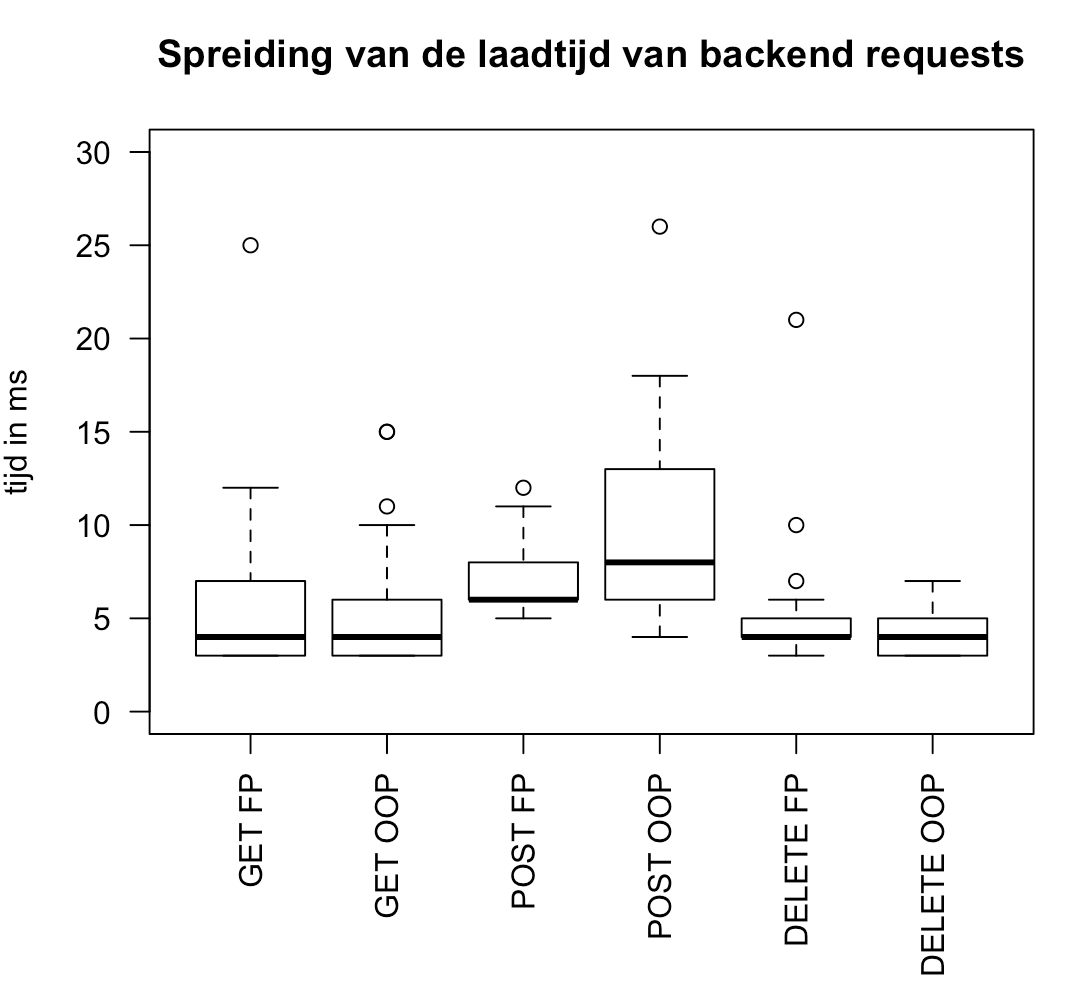
\includegraphics[width=\linewidth]{img/performantie-backend.png}
    \caption{Performantie Backend}
    \label{fig:performantiebackend}
  \end{figure}

  Ook hier lijkt op het eerste zicht de performantie gelijk. De enige afwijking die te zien is op de boxplot is die van de POST requests, nl. de spreiding en het gemiddelde van de POST request bij de OOP backend is iets groter. Het berekenen van de p-waarde echter (0,1711) toont weer aan dat deze statistisch niet significant verschillend zijn, idem voor de GET requests (0,406) en DELETE requests (0,1198). De gemiddeldes voor FP backend request bedragen 6.9 (GET), 8.8 (POST) en 5.13 (DELETE). Voor OOP zijn de gemiddeldes 5.5 (GET), 15.23 (POST), 4.1 (DELETE).

\subsection{Complexiteit}
Om de complexiteit te kunnen berekenen van software kan er gebruikt gemaakt worden van een cyclomatic complexity metriek. Deze is echter moeilijk toe te passen op webapplicaties aangezien er nog andere factoren meespelen dan enkel de code en bovendien zijn deze applicaties te klein om deze metriek te kunnen berekenen. De meeste functies krijgen gewoonweg een cyclomatic complexity van 1 toegekend, wat in principe wil zeggen dat de functie niet complex is. Een andere metriek voor complexiteit is de maintainability index. Deze geeft aan hoe makkelijk het is om bepaalde stukken code te onderhouden. Hoe groter de waarde, hoe makkelijker het is om de code te onderhouden. In het algemeen betekent een waarde vanaf 100 dat de code goed onderhoudbaar is. De gemiddelde maintainability index voor de FP backend bedraagt 126,51 en die voor de OOP backend 136,24, wat ook toont dat de complexiteit in beide applicaties laag ligt. Opvallend is dat de index bij OOP toch iets hoger ligt, onderhoudbaarheid is dan ook een belofte van het volgen van het functioneel programmeren paradigma. 
